\documentclass{article}
\usepackage{amsmath}
\usepackage{graphicx}
\usepackage{xcolor}
\usepackage{listings}
\usepackage{geometry}
\usepackage{circuitikz}
\geometry{legalpaper, left=20mm,top=25mm}
\usepackage[utf8]{inputenc}
\renewcommand{\familydefault}{\sfdefault}
\renewcommand{\baselinestretch}{1.5}

\definecolor{numberingcolor}{rgb}{1,0,0}
\definecolor{backgroundcolour}{rgb}{0.97,0.97,0.97}

\lstdefinestyle{CodeStyle}{
  backgroundcolor=\color{backgroundcolour},
  numberstyle=\tiny\color{numberingcolor},
  basicstyle=\ttfamily\footnotesize,
  breakatwhitespace=false,         
  breaklines=false,                 
  captionpos=b,                    
  keepspaces=true,                 
  numbers=left,                    
  numbersep=5pt,                  
  showspaces=false,                
  showstringspaces=false,
  showtabs=false,                  
  tabsize=7
}
\lstset{style=CodeStyle}

\title{EE3113 Homework Assignment-3}
\author{Krishna Srikar Durbha}
\date{EE18BTECH11014}

\begin{document}
\maketitle
\textbf{Note:} Mathematical Explanations for some of the questions are at the end. 
\section{1. Impact of Sizing on Performance}
\textbf{Specifications:}
\begin{align}
    V_{M} = \frac{V_{DD}}{2}\\
    V_{DD} = 1.8 \text{ Volts}\\
    V_{M} = 0.9 \text{ Volts}
\end{align}
For the above condition to be satisfied, $\frac{W}{L}$ ratios should be,
\begin{align}
    W_{n} = 0.18\mu \text{m}\\
    L_{n} = 0.18\mu \text{m}\\
    W_{p} = 1.165\mu \text{m}\\
    L_{p} = 0.18\mu \text{m}
\end{align}
\subsection{1a}
\subsubsection{i}
\textbf{SPICE Netlist}:
\begin{lstlisting}
Question-1a(i)

* Model
.include "TSMC180.lib"
.model nch_tt nmos
.model pch_tt pmos

* Circuit
Vdd	S	0	DC	1.8
MP	D	G	S	S	pch_tt W=1.165u L=0.18u
MN	D	G	0	0	nch_tt W=0.18u L=0.18u
Vin	G	0	PULSE(0	1.8 0 0 0 0.5n 1n 0)

* Analysis
.tran	0.1p	1n

* Results
.control
run
plot	V(D)	V(G)
.endc

.end
\end{lstlisting}
\textbf{Results:}
\begin{figure}[!ht]
    \centering
    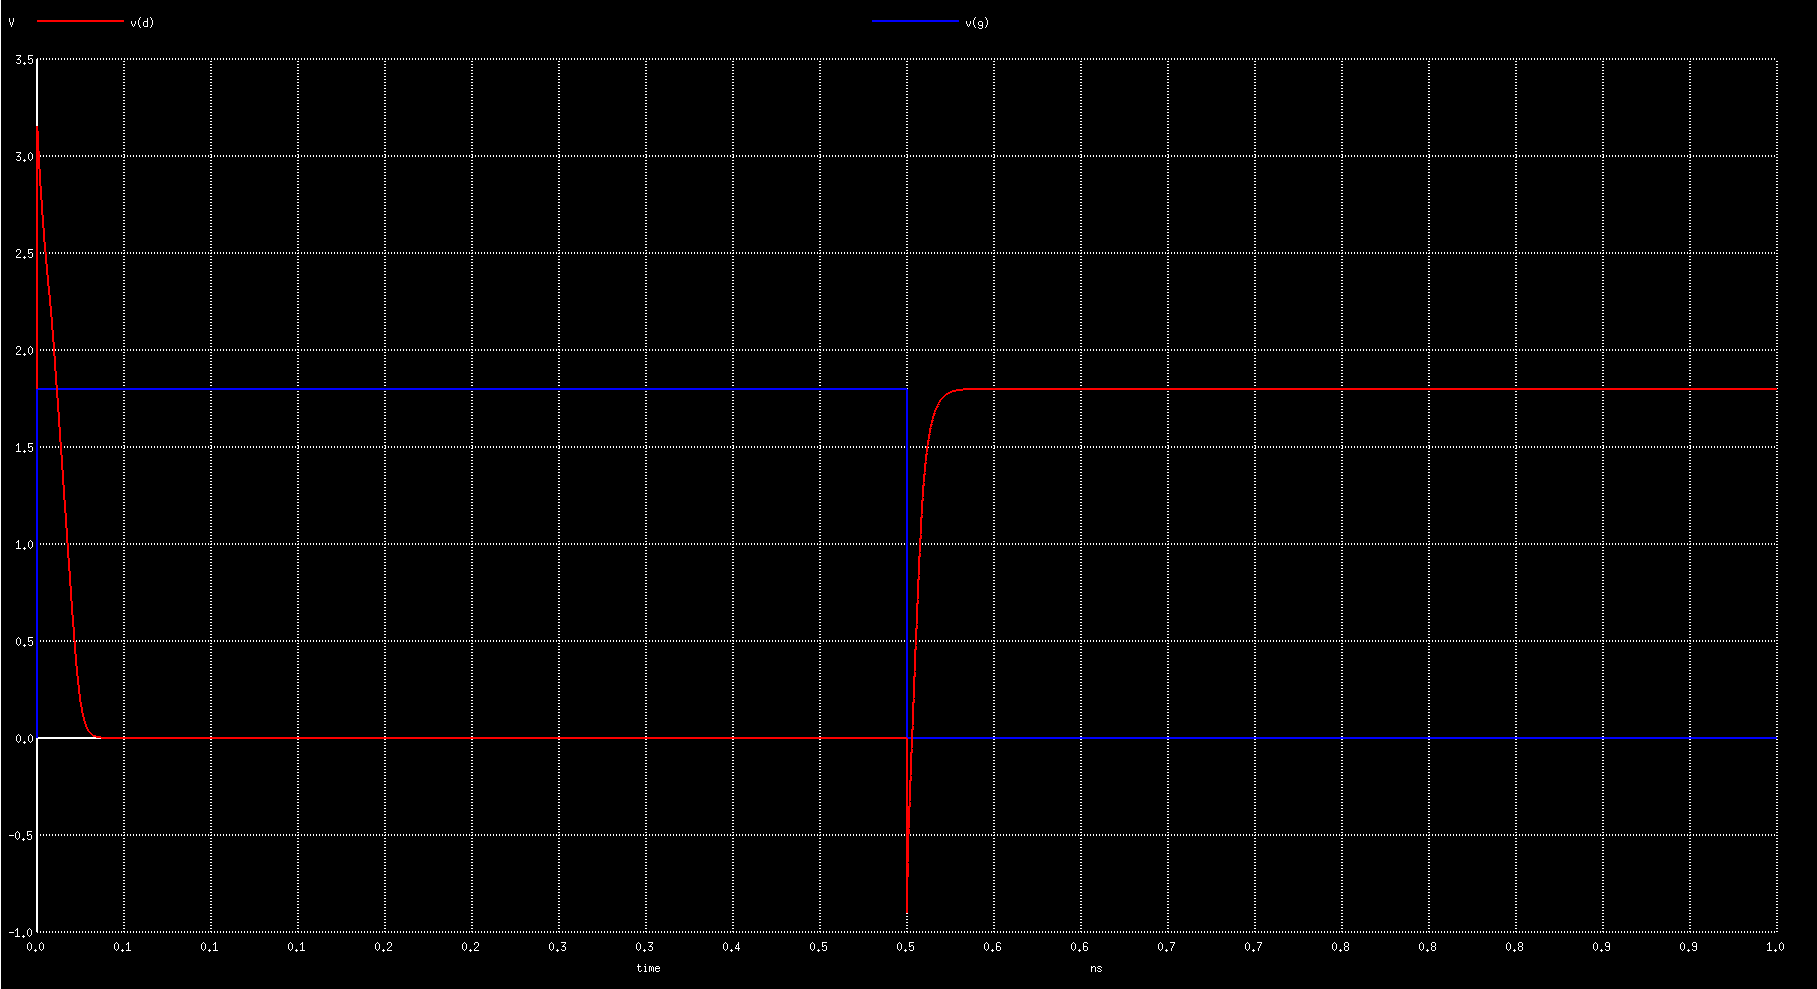
\includegraphics[scale=0.23]{Images/1ai.png}
    \caption{When $\frac{W}{L}$ ratios are as per Specifications and when there is no External-Load $C_{L}$.}
\end{figure}\\
\textbf{Variation of $t_{p}$ with Scaling Factor $S$:}\\
As, the part of Scaling, Width of both N-MOSFET and P-MOSFET are increased by a factor of $S$.
\begin{center}
    \begin{tabular}{ |p{1.5cm}|p{3cm}|p{3cm}|p{5cm}| } 
    \hline
    $S$ & $t_{pHL}$ (in sec) & $t_{pLH}$ (in sec) & $t_{p} = \frac{t_{pLH} + t_{pHL}}{2}$ (in sec)\\ 
    \hline
    \hline
    1 & 1.84211 \times 10^{-11} & 0.7018 \times 10^{-11} & 1.271955 \times 10^{-11}\\
    \hline
    2 & 2.1519 \times 10^{-11} & 0.63 \times 10^{-11} & 1.39095 \times 10^{-11}\\
    \hline
    5 & 2.6744 \times 10^{-11} & 0.814 \times 10^{-11} & 1.7442 \times 10^{-11}\\
    \hline
    7.5 & 2.75862 \times 10^{-11} & 0.8046 \times 10^{-11} & 1.78161 \times 10^{-11}\\
    \hline
    10 & 2.7381 \times 10^{-11} & 0.8333 \times 10^{-11} & 1.7857 \times 10^{-11}\\
    \hline
    \end{tabular}
\end{center}
\vspace{0.2in}
\qquad When there is no External Load, the Propagation Delay ($t_{p}$) is almost negligible. So, there is no variation of $t_{p}$ by changing Scaling Factor($S$). When no External-Load is present Capacitance in Propagation Delay expression would be Drain Capacitance of both N-MOSFET and P-MOSFET whose values are very small. So, change in $t_{p}$ will almost be negligible. 

\pagebreak
\subsubsection{ii}
\textbf{SPICE Netlist}:
\begin{lstlisting}
Question-1a(ii)

* Model
.include "TSMC180.lib"
.model nch_tt nmos
.model pch_tt pmos

* Circuit
Vdd	S	0	DC	1.8
MP	D	G	S	S	pch_tt W=1.165u L=0.18u
MN	D	G	0	0	nch_tt W=0.18u L=0.18u
Vin	G	0	PULSE(0	1.8 0 0 0 0.5u 1u 0)
C	D	0	20p

* Analysis
.tran	1n	2u

* Results
.control
run
plot	V(D)	V(G)
.endc

.end
\end{lstlisting}
\textbf{Results:}\\
\begin{figure}[!ht]
    \centering
    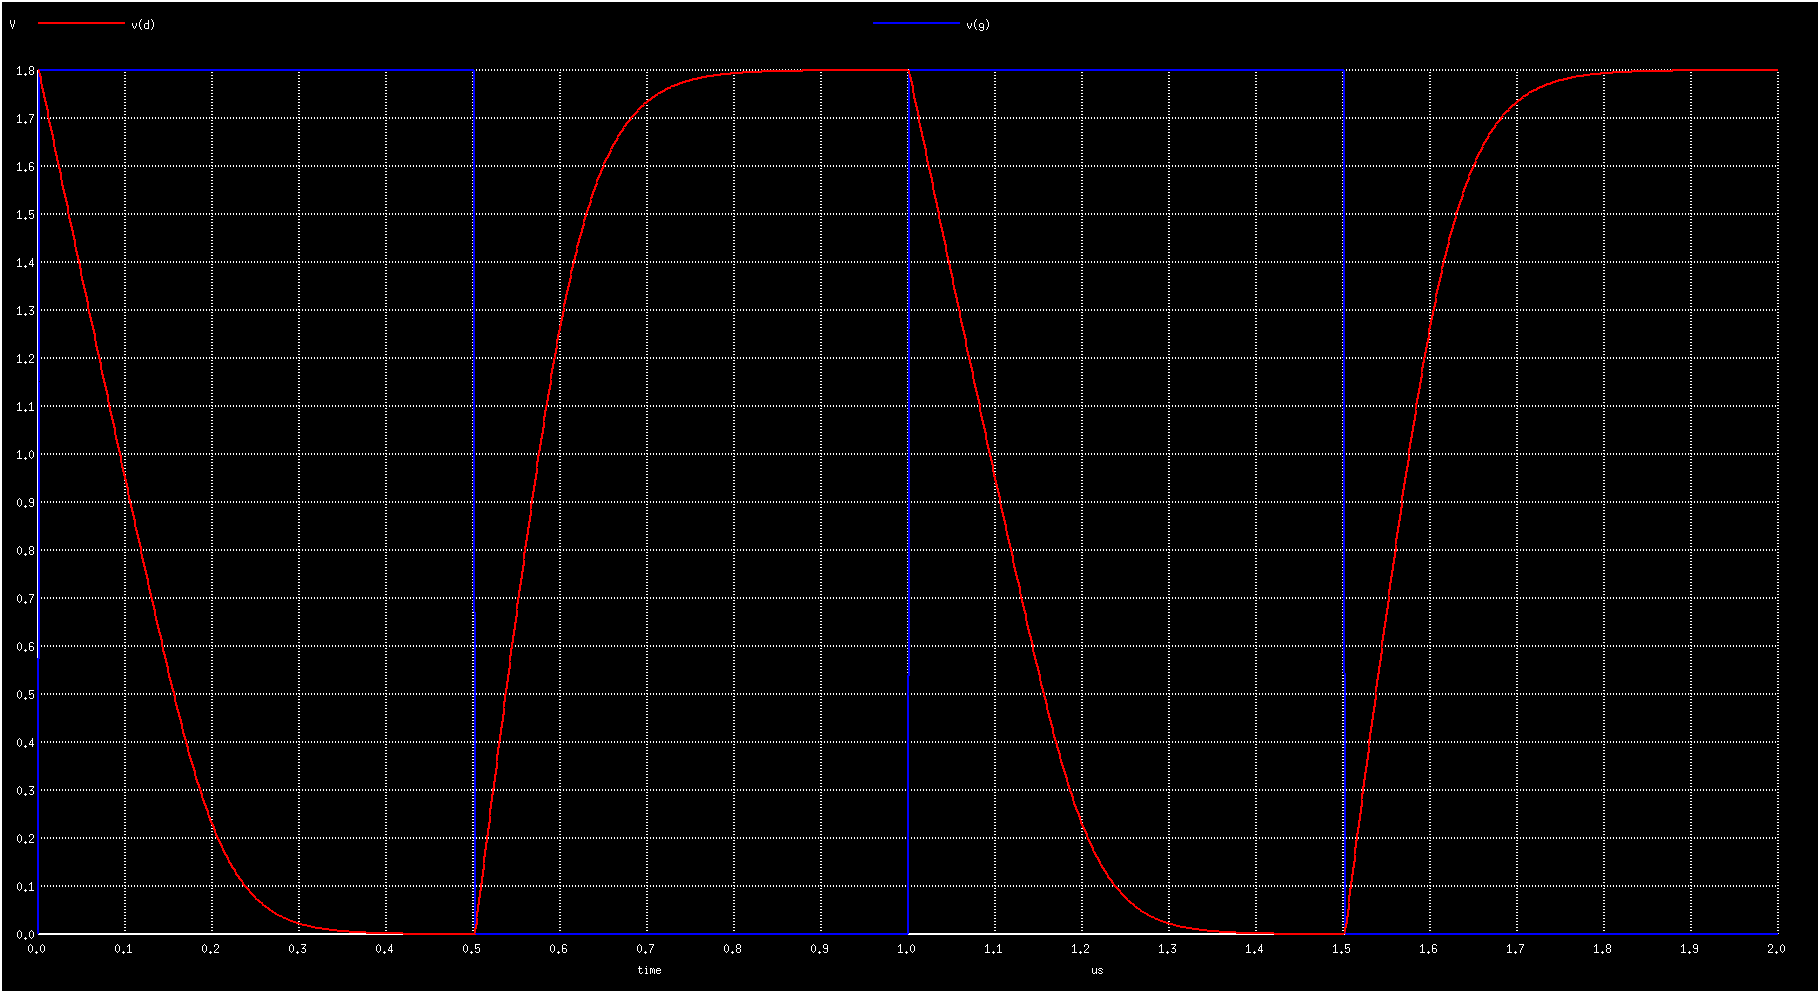
\includegraphics[scale=0.23]{Images/1aii.png}
    \caption{When $\frac{W}{L}$ ratios are as per Specifications and when there is External-Load $C_{L} = 20pF$.}
\end{figure}
\\
\textbf{Variation of $t_{p}$ with Scaling Factor $S$:}\\
As, the part of Scaling, Width of both N-MOSFET and P-MOSFET are increased by a factor of $S$.
\begin{center}
    \begin{tabular}{ |p{1.5cm}|p{3cm}|p{3cm}|p{5cm}| } 
    \hline
    $S$ & $t_{pHL}$ (in sec) & $t_{pLH}$ (in sec) & $t_{p} = \frac{t_{pLH} + t_{pHL}}{2}$ (in sec)\\ 
    \hline
    \hline
    1 & 1.07143 \times 10^{-7} & 0.64881 \times 10^{-7} & 0.86012 \times 10^{-7}\\
    \hline
    2 & 0.692982 \times 10^{-7} & 0.34211 \times 10^{-7} & 0.517546 \times 10^{-7}\\
    \hline
    4 & 0.408046 \times 10^{-7} & 0.17816 \times 10^{-7} & 0.293103 \times 10^{-7}\\
    \hline
    6 & 0.280702 \times 10^{-7} & 0.12281 \times 10^{-7} & 0.201756 \times 10^{-7}\\
    \hline
    8 & 0.219298 \times 10^{-7} & 0.0965 \times 10^{-7} & 0.157899 \times 10^{-7}\\
    \hline
    10 & 0.184211 \times 10^{-7} & 0.07018 \times 10^{-7} & 0.1271955 \times 10^{-7}\\
    \hline
    \end{tabular}
\end{center}
\vspace{0.2in}
\textbf{Plots:}
\begin{figure}[!ht]
    \centering
    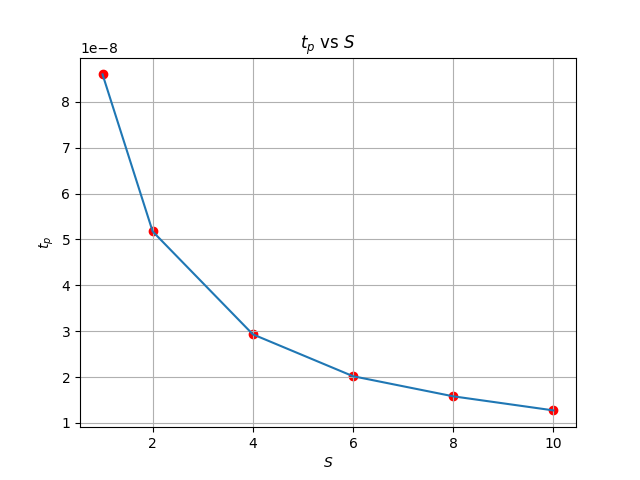
\includegraphics[scale=0.75]{Images/1a.png}
    \caption{$t_{p}$ vs $S$}
\end{figure}\\
As Scaling increases, MOSFET Resistance decreases, which further decreases, $t_{p}$.

\subsection{1b}
\textbf{Impact of $W_{p}$:}\\
$W_{p}$ effects $t_{pLH}$ as Critical Path while charging of Load Capacitor happens through P-MOSFET.\\
\textbf{Variation of $t_{p}$ by scaling only P-MOSFET by a factor $S$:}
\begin{center}
    \begin{tabular}{ |p{1.5cm}|p{3cm}|p{3cm}|p{5cm}| } 
    \hline
    $S$ & $t_{pHL}$ (in sec) & $t_{pLH}$ (in sec) & $t_{p}$ (in sec)\\ 
    \hline
    \hline
    1 & 1.07143 \times 10^{-7} & 0.64881 \times 10^{-7} & 0.86012 \times 10^{-7}\\
    \hline
    2 & 1.06322 \times 10^{-7} & 0.336392 \times 10^{-7} & 0.699806 \times 10^{-7}\\
    \hline
    4 & 1.06322 \times 10^{-7} & 0.16667 \times 10^{-7} & 0.614945 \times 10^{-7}\\
    \hline
    6 & 1.06322 \times 10^{-7} & 0.12069 \times 10^{-7} & 0.591955 \times 10^{-7}\\
    \hline
    8 & 1.06322 \times 10^{-7} & 0.08621 \times 10^{-7} & 0.574715 \times 10^{-7}\\
    \hline
    10 & 1.06322 \times 10^{-7} & 0.07471 \times 10^{-7} & 0.568965 \times 10^{-7}\\
    \hline
    \end{tabular}
\end{center}\\
\textbf{Results:}\\
\pagebreak
\begin{figure}[!ht]
    \centering
    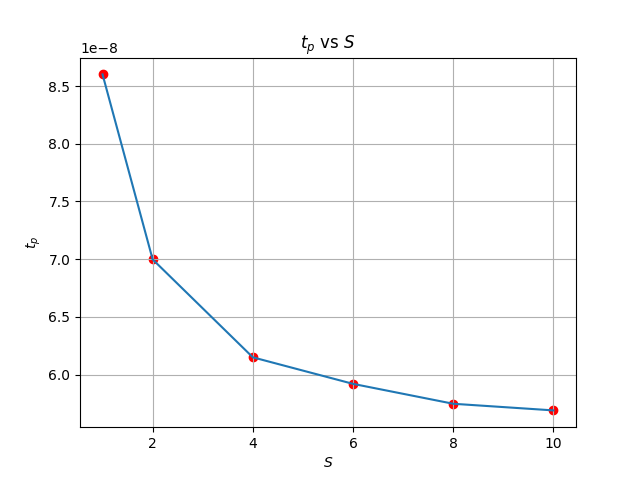
\includegraphics[scale=0.75]{Images/1b1.png}
    \caption{$t_{p}$ vs $S$}
\end{figure}\\
\textbf{Impact of $W_{n}$:}\\
$W_{n}$ effects $t_{pHL}$ as Critical Path while discharging of Load Capacitor happens through N-MOSFET.\\
\textbf{Variation of $t_{p}$ by scaling only N-MOSFET by a factor $S$:}
\begin{center}
    \begin{tabular}{ |p{1.5cm}|p{3cm}|p{3cm}|p{5cm}| } 
    \hline
    $S$ & $t_{pHL}$ (in sec) & $t_{pLH}$ (in sec) & $t_{p} = \frac{t_{pLH} + t_{pHL}}{2}$ (in sec)\\ 
    \hline
    \hline
    1 & 1.07143 \times 10^{-7} & 0.64881 \times 10^{-7} & 0.86012 \times 10^{-7}\\
    \hline
    2 & 0.695402 \times 10^{-7} & 0.65517 \times 10^{-7} & 0.675286 \times 10^{-7}\\
    \hline
    4 & 0.408046 \times 10^{-7} & 0.65517 \times 10^{-7} & 0.531608 \times 10^{-7}\\
    \hline
    6 & 0.281609 \times 10^{-7} & 0.65517 \times 10^{-7} & 0.4683895 \times 10^{-7}\\
    \hline
    8 & 0.218391 \times 10^{-7} & 0.65517 \times 10^{-7} & 0.4367805 \times 10^{-7}\\
    \hline
    10 & 0.172414 \times 10^{-7} & 0.65517 \times 10^{-7} & 0.413792 \times 10^{-7}\\
    \hline
    \end{tabular}
\end{center}
\textbf{Results:}
\begin{figure}[!ht]
    \centering
    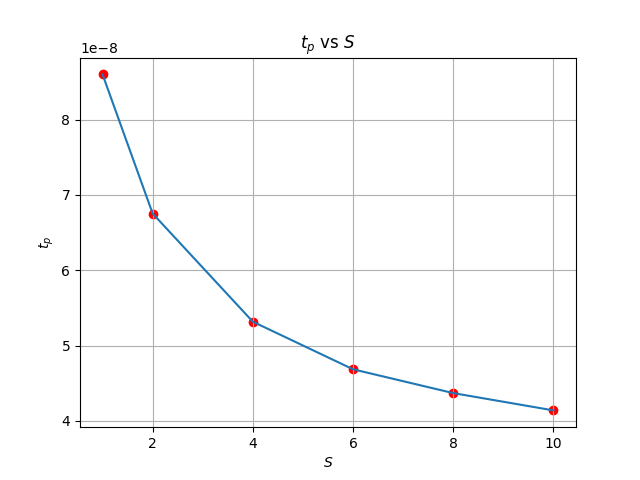
\includegraphics[scale=0.75]{Images/1b2.png}
    \caption{$t_{p}$ vs $S$}
\end{figure}

\section{Ring Oscillator}
\textbf{Specifications:}\\
7-Stage Ring Oscillator by cascading Unit Inverters.
\subsection{2a}
\textbf{SPICE Netlist:}
\begin{lstlisting}
Question-2

* Model
.include "TSMC180.lib"
.model nch_tt nmos
.model pch_tt pmos

* Circuit
Vdd	S	0	DC	1.8
MP1	D1	D7	S	S	pch_tt W=1.165u L=0.18u
MN1	D1	D7	0	0	nch_tt W=0.18u L=0.18u
C1	D1	0	20p
MP2	D2	D1	S	S	pch_tt W=1.165u L=0.18u
MN2	D2	D1	0	0	nch_tt W=0.18u L=0.18u
C2	D2	0	20p
MP3	D3	D2	S	S	pch_tt W=1.165u L=0.18u
MN3	D3	D2	0	0	nch_tt W=0.18u L=0.18u
C3	D3	0	20p
MP4	D4	D3	S	S	pch_tt W=1.165u L=0.18u
MN4	D4	D3	0	0	nch_tt W=0.18u L=0.18u
C4	D4	0	20p
MP5	D5	D4	S	S	pch_tt W=1.165u L=0.18u
MN5	D5	D4	0	0	nch_tt W=0.18u L=0.18u
C5	D5	0	20p
MP6	D6	D5	S	S	pch_tt W=1.165u L=0.18u
MN6	D6	D5	0	0	nch_tt W=0.18u L=0.18u
C6	D6	0	20p
MP7	D7	D6	S	S	pch_tt W=1.165u L=0.18u
MN7	D7	D6	0	0	nch_tt W=0.18u L=0.18u
C7	D7	0	20p


* Analysis
.tran	20p	20u

* Results
.control
run
plot	V(D7)
.endc

.end
\end{lstlisting}
Time-Period and Frequency of Oscillations:\\
\begin{align}
    T = 1.8133 \times 10^{-6} \text{ sec}\\
    f = 0.552080515 \text{ MHz}
\end{align}
\textbf{Results:}\\
\begin{figure}[!ht]
    \centering
    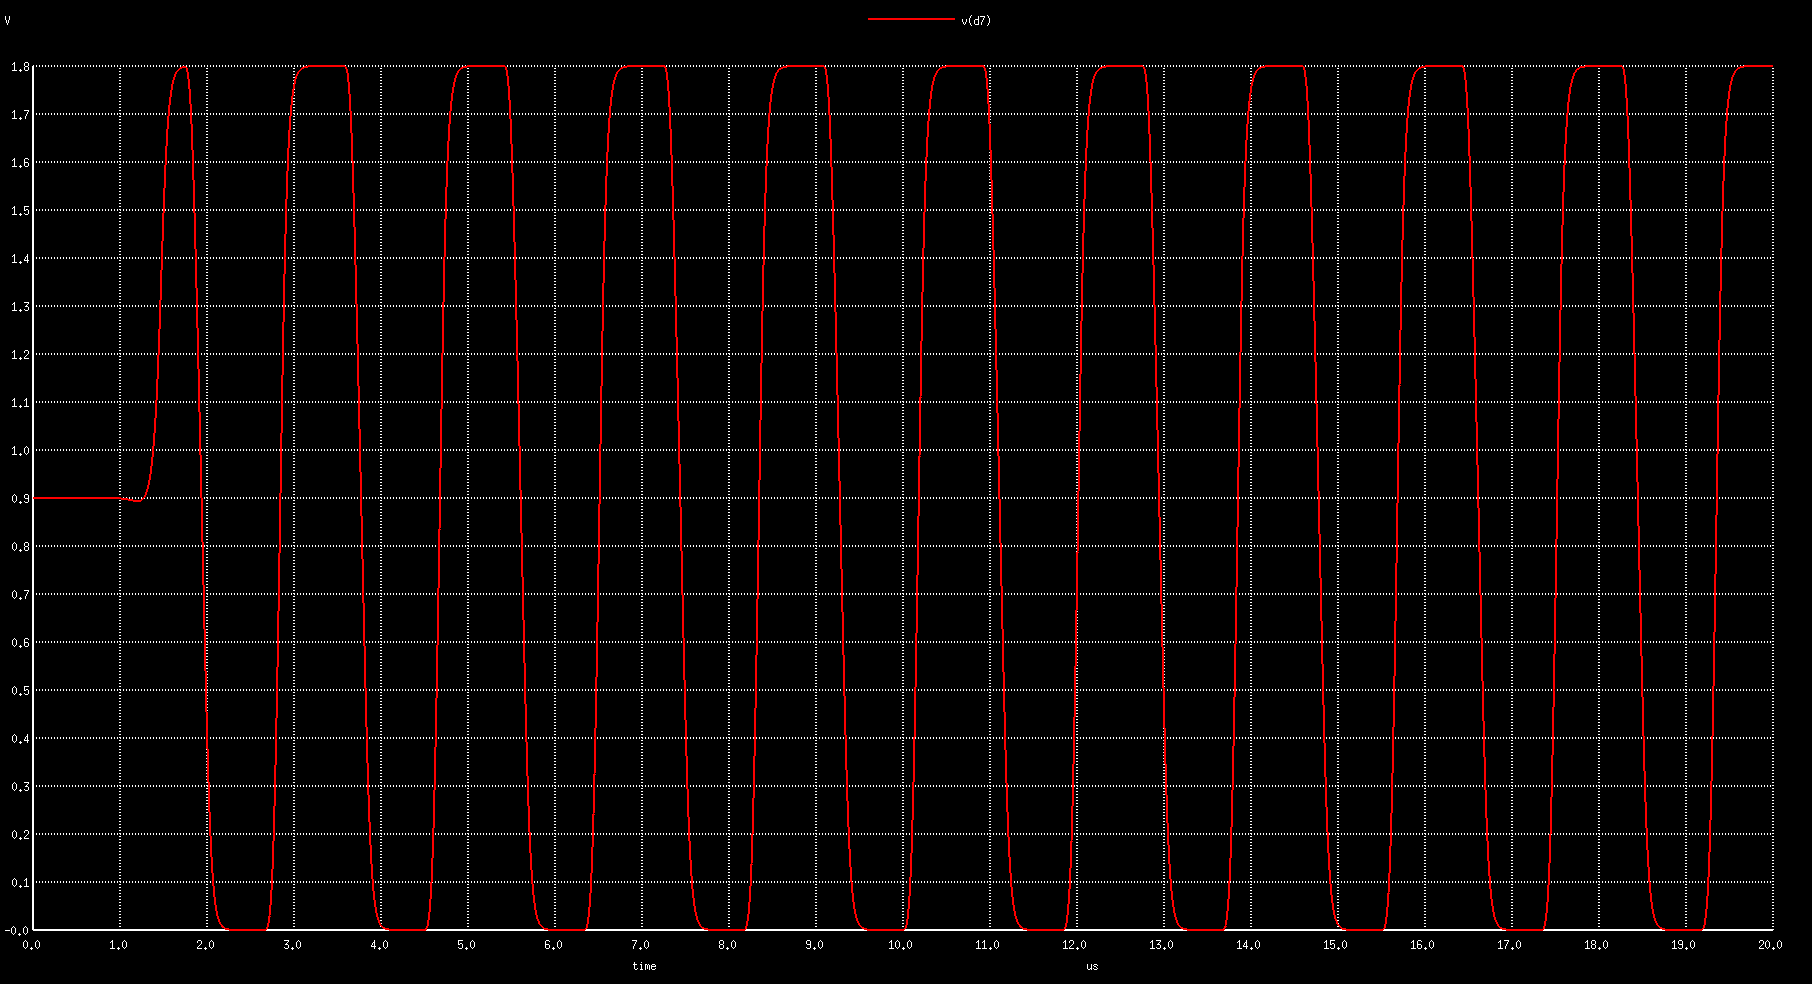
\includegraphics[scale=0.23]{Images/2a.png}
\end{figure}\\

\subsection{2b}
\begin{align}
    t_{pLH} = 0.16981 \times 10^{-6} \text{ s}\\
    t_{pHL} = 0.16981 \times 10^{-6} \text{ s} \\
    t_{p} = 0.16981 \times 10^{-6} \text{ s}
\end{align}

\subsection{2c}
By sizing up the the MOSFETs, Resistances of both P-MOS and N-MOS decrease which leads to decrease in Propagation Delay. This also increases Frequency of Oscillations.

\subsection{2d}
\qquad Instead of directly connecting the Output of Ring Oscillator to its Input, we can use a Switch to Start and Stop Oscillations.

\qquad When Switch is \textbf{ON}, there will be oscillations. When Switch is \textbf{OFF}, Output will remain in previous state. 
\end{document}